% !TEX program = xelatex -> bibtex -> xelatex*2

\documentclass[12pt]{ctexart}  
% ctexart支持中文编译文档
%最后全部翻译成英文后可以选择改成article,然后用pdflatex编译,还可以检验一下是不是没有中文了嘿嘿( •̀ ω •́ )✧
%官方要求字号不小于 12 号,此处选择 12 号字体
\usepackage{makecell} % Added for \makecell support
\usepackage{graphicx}
\usepackage{xcolor}
\usepackage{background}

\CTEXsetup[format={\Large\bfseries}]{section} %在ctexart中,一级标题是居中的,这里改成左对齐

%% 本模板不需要填写年份,以当前电脑时间自动生成

%% 请在以下的方括号中填写队伍控制号
\usepackage[2615409]{ldmcm}  % 载入ldmcm模板文件
\problem{B}  % 请在此处填写题号

%%字体选择
%\usepackage{mathptmx}  % 这是 Times 字体,中规中矩 
\usepackage{mathpazo}  % 这是 COMAP 官方杂志采用的更好看的 Palatino 字体,可替代以上的 mathptmx 宏包

%%几处小修改,如无特殊需求可不做更改
\newcommand{\upcite}[1]{\textsuperscript{\textsuperscript{\cite{#1}}}}%这是参考文献引用上标的命令
\graphicspath{{img/}}          % 此处{img/}为相对路径,注意加上“/”
\let\itemize\compactitem
\let\enditemize\endcompactitem%解决列表环境中行距过大的问题

\title{Here is Your Title}  % 标题

% 如需要修改题头(默认为 MCM /ICM),请使用以下命令(此处修改为 MCM)
%\renewcommand{\contest}{MCM}

\usepackage{lastpage}  % 支持 \pageref{LastPage}

\usepackage{siunitx}

% ----------------------------------------------文档开始---------------------------------------------------------
\begin{document}
\backgroundsetup{contents={}} 
% 此处填写摘要内容-----------摘要摘要摘要摘要摘要摘要摘要摘要摘要摘要摘要摘要摘要摘要摘要摘要摘要摘要摘要摘要摘要
\begin{abstract}
	%第一段:2句话背景+2句话概括全文完成的任务

	\textbf{The construction of a lunar colony} supporting 100,000 inhabitants by 2050 poses significant challenges in transporting massive construction materials from Earth. Efficient, cost-effective, and environmentally sustainable delivery methods are essential. 
	Our mission focused on analyzing and optimizing transport strategies combining Space Elevator technology and traditional rocket launches to fulfill these requirements.

	%第二段:总结我们用了什么模型	
	We developed three models. \textbf{Model I} is a static benchmark that uses data on payload capacities, launch frequencies, and costs to evaluate three scenarios: \textbf{Space Elevator only}, \textbf{Traditional Rocket only}, and a \textbf{static hybrid mode}. This model provides baseline comparisons of duration and costs, showing hybrid strategies improve feasibility and efficiency over single-mode approaches. Compared to the pure space elevator mode, it reduces construction time by 25\%, while cutting costs by 63.4\% relative to the pure traditional rocket mode.

	\textbf{Model II} extends to a \textbf{dynamic adjusted} framework, modeling transport ratios as piecewise constants over 50 intervals, incorporating technological progress and cost reductions. Using a \textbf{Stage-wise Extended Search Algorithm} and \textbf{Greedy Marginal Cost Method}, this model optimizes allocation dynamically, achieving better balance among time, cost, and environmental impact, which gains the smallest composite score (0.471).

	\textbf{Model III} incorporates \textbf{stochastic} uncertainties such as rocket launch failures and tether sway using probabilistic approaches to adjust effective capacities and costs, enhancing model realism and robustness.

	%灵敏度与稳健性分析
	Finally, \textbf{sensitivity} and \textbf{robustness} analyses quantify the effect of key parameters including system capacity, failure probabilities, and clean energy use. Results validate that the dynamic hybrid approach consistently offers superior performance across efficiency, cost, and sustainability objectives, recommending it as the optimal strategy for lunar material transportation.

	% 美赛论文中无需注明关键词。若一定要使用,
	% 请将以下两行的注释号 '%' 去除,以使其生效
	\vspace{5pt}
	\textbf{Keywords}: Space Elevator, Rocket, Hybrid Transport Strategy, Dynamic Optimization, Pareto Frontier Analysis, Stochastic Modeling, Sensitivity Analysis.

\end{abstract}

\maketitle  % 生成 Summary Sheet------------------------------------

\tableofcontents  % 生成目录


% -----------------------------------------正文开始-----------------------------------------------------------------------------------------------------------------------------------


%==============第一部分===引入=============================================================
\section{Introduction}
\subsection{Problem Background}%问题背景问题背景问题背景问题背景问题背景问题背景---------------------------------
%美赛一定要多上图,清晰直观,并且格式上最好是矢量图,例如pdf,而不是位图,例如jpg,png等,在形式上最好是组图,下面列出了利用\verb|subfigure|实现的
%\verb|1x2,1x3,2x2|的几种组图:
Some researchers envision an electrically powered Space Elevator System, offering scalable infrastructure for interplanetary logistics, commerce, and exploration.

In its mature form, the system consists of three Galactic Harbours evenly spaced 120° along the equator. Each harbour has one Earth port linked to two 100,000-km tethers leading to apex anchors. Cooperating, multiple elevators can routinely transport large payloads from Earth to geosynchronous orbit (GEO) and onward to the anchors, where they are transferred to rockets with significantly reduced propellant needs.

%% 这是问题背景的概念图
\begin{figure}[htbp]
	\centering
	\begin{subfigure}[b]{.8\textwidth} %设置缩放比例,这里的.5代表缩放为原来的50%
		\includegraphics[width=\textwidth]{img/background.png}
		\caption*{}
		\label{}
	\end{subfigure}
	\caption{problem background}\label{background}
\end{figure}

Based on this system, the Moon Colony Management (MCM) Agency plans to build a lunar colony accommodating 100,000 people, starting in 2050 after the elevator system’s completion. It is also considering traditional rockets to supply construction materials and daily provisions. Currently, there are ten rocket launch sites worldwide.

As shown in figure\ref{background},the schematic of the Space Elevator System and Moon Colony is illustrated above.

%\subsection{Problem Background}%问题重述与文献综述选一个------------------------------------------------------------------------
\subsection{Literature Review} % 文献综述-----------------
Three major problems are discussed in this paper, which are:
\begin{itemize}
	\item First and foremost, it is necessary to analyze three distinct scenarios for delivering the 100 million metric tons of materials required for the construction of the 100,000-person Moon Colony. The three scenarios to be considered include: (a) SE: relying solely on the three Galactic Harbors of the Space Elevator System; (b) TR: relying exclusively on traditional rocket launches from selected existing space facilities; and (c) adopting a hybrid delivery strategy that combines the SE and the TR. For each scenario, a comprehensive assessment of the project duration and total cost must be conducted.
	
	\item Second, the robustness of the proposed material delivery solutions needs to be evaluated under the condition that transportation systems are not in perfect working order, such as rocket launch failures, sway amplitude and wind speed.

	\item Third, the water demand of the 100,000-person Moon Colony over a one-year period after it is fully operational must be systematically investigated. Based on the established material transportation model , the additional costs and extended timeline required to be ensured to satisfy the colony has sufficient water supply for one full year.
	
	\item  Finally, the environmental impacts on Earth associated with achieving the 100,000-person Moon Colony under different conditions. On this basis, we should adjust the model to the established delivery model should be proposed to minimize the adverse environmental impacts on Earth.
\end{itemize}

%月球水
A literatrue\upcite{jones2015water} reviews the water demand of lunar bases: the basic domestic water consumption 
is 4.17 kg per person per day, covering drinking, sanitation and other uses. A daily wastewater yield of 5.57 kg per person is generated, 
with condensed water and urinary wastewater recoverable as supplementary water sources.
 The relevant water system technologies are adaptable to the gravitational environments of the Moon(data based on NASA Exploration Program assumptions).

%太空电梯
A literature\upcite{smitherman2000space} confirm that space elevators have a solid technological and economic feasibility 
basis. High-strength materials such as carbon nanotubes meet the theoretical strength requirements; Low Earth Orbit (LEO) space elevators 
are technologically feasible with supporting propulsion solutions.

%地月运输
In the literature\upcite{ishimatsu2016generalized}, a generalized multi-commodity network flow (GMCNF) model has been proposed to optimize logistics within the Earth–Moon–Mars system.
 It incorporates multi-commodity flows like propellant, crew, and equipment.

%火箭污染
A literatrue\upcite{ross2014radiative}shows:Rocket exhaust produces positive radiative forcing (RF), primarily due to black carbon (BC) and alumina particles.
Current global RF from rocket launches is estimated at 16±8$mWm^{-2}$, with BC accounting for 70 percents of this value.

\subsection{Our work}%-----------------------------------------------------------
\begin{figure}[htbp]
	\centering
	\begin{subfigure}[b]{1\textwidth} %设置缩放比例,这里的.5代表缩放为原来的50%
		\includegraphics[width=\textwidth]{img/our_work.png}
		\caption*{}
		\label{}
	\end{subfigure}
	\caption{our work}\label{ourwork}
\end{figure}

\begin{enumerate}[\bfseries 1.]
	\item \textbf{We do model construction.} We build a series of mathematical models to analyze and optimize the lunar material delivery system. Starting from a static baseline model, we compare three transportation scenarios. On this basis, we further establish a dynamic extended model that allows the transportation ratio $\alpha_i$ to evolve over time, incorporating technical progress and cost reduction. Finally, we introduce stochastic elements to ensure the model reflects realistic uncertainty.
	\item \textbf{We do extended tasks.} We integrate additional requirements into the core framework. The water demand model quantifies the annual net water requirement under different recycling efficiencies, while the environmental impact model evaluates $CO_2$ and black carbon emissions from rockets, as well as energy use from the Space Elevator. This extension allows the model to balance cost, time, and ecological sustainability.
	\item \textbf{We do model solving and evaluation.} We design a Stage-wise Extended Search Algorithm (SESA) combined with a Greedy Marginal Cost Method (GMCM) to solve the nonlinear, multi-objective optimization problem. Pareto front analysis and knee-point detection are applied to identify optimal trade-offs between construction time, cost, and environmental impact. Additionally, sensitivity and robustness analyses verify model reliability and demonstrate that the dynamic hybrid strategy achieves the best performance among all schemes.
\end{enumerate}
%===========================第二部分==模型准备==========================================================
\section{Preparation of the Models}
\subsection{Assumptions and Explanations}
%为了简化问题,我们做出了以下假设,其中每一条都有对应的合理解释
To simplify the problem, we made the following assumptions, each of which has a corresponding reasonable explanation.
\begin{itemize}
	\item \textit{\textbf{Assumption 1:}}Consistency of materials: Materials are treated as quasi-continuous fluids and can be infinitely subdivided.
	\\$\hookrightarrow$ \textit{\textbf{Explanation:}}The project involves a large volume of materials, which are treated as fluids to align with scheduling logic.
	\item \textit{\textbf{Assumption 2:}}Imperfect state parameters: TR transmission failure probability of 1%, which will decrease to 0.1% with technological advancement.
	\\$\hookrightarrow$ \textit{\textbf{Explanation:}}Based on historical aerospace engineering data and the scenario of the question, a reasonable setting is established.
	\item \textit{\textbf{Assumption 3:}}The cost of an apex rocket launch failure is not counted.
	\\$\hookrightarrow$ \textit{\textbf{Explanation:}}Due to the unknown payload capacity of the apex stage rocket, cost fluctuations are factored into the original cost.
\end{itemize}
%这里只列出了主要的假设,其他假设会在专门的小节中单独讨论
Additional assumptions are made to simplify analysis for individual sections. These assumptions will be discussed at the appropriate locations.

\subsection{Notations}%-----------------------------------------------------------------------------------
% 三线表(可以直接在excel里编辑好然后用excel2latex插件插入)

Table \ref{tb:notation} lists some important mathematical notations used in this paper.
\begin{table}[htbp]%----------------------------------------------
	\begin{center}
		\caption{Notations used in this paper}
		\begin{tabular}{cl}
			\toprule[1.5pt]
			\multicolumn{1}{m{4cm}}{\centering \textbf{Symbol}}
			                      & \multicolumn{1}{m{10cm}}{\textbf{ Description} }                       \\
			\midrule
			$\alpha_i$            & SE transport proportion interval at stage i(piecewise constant $\alpha(t)$)                      \\
			$q_i$                 & Average capacity at stage i                                                  \\
			$M_{tot}$             & Total construction materials                                                           \\
			$\kappa_{SE,total}$   & SE system total annual capacity                                                         \\
			$m_{load}$            & TR single-payload benchmark value                                                    \\
			$f_{TR}(j)$           & Annual maximum launch frequency of the j-th TR launch site                                            \\
			$C_{fix}^{SE}$        & SE system total fixed cost                                                       \\
			$c_{var}^{SE}$        & SE unit variable cost + apex rocket unit mass launch cost                                \\
			$c_{launch}$          & TR single launch cost                                                         \\
			$P_{pop}$             & Lunar colony population                                                         \\
			$w_{per}$             & Daily per capita water consumption                                                           \\
			$\gamma$              & Water resource cycle efficiency                                                         \\
			$\eta_{clean}$        & Clean energy utilization rate                                                         \\
			$Q_{SE}(i)$           & Cumulative transport volume for the previous i intervals                                                  \\
			$Q_{TR}(i)$           & Cumulative transport volume for the previous i intervals of TR                                                  \\
			$D(i)$                & Cumulative damage factor for the i-th interval of SE                                                \\
			$\kappa_{SE}'(i)$     & Effective transport capacity of SE in the i-th interval (non-perfect state)                                     \\
			$\kappa_{TR}'(i)$     & Effective transport capacity of TR in the i-th interval (non-perfect state)                                     \\
			$f_{cost}$            & Total lifecycle cost                                                       \\
			$T$            & Total construction period                                                                 \\
			$E$             & Comprehensive environmental impact index                                                       \\
			\bottomrule[1.5pt]
		\end{tabular}\label{tb:notation}
		\begin{tablenotes}
			\footnotesize
			\item[*] *Some variables are not listed here and will be discussed in detail in each section. %此处加入注释*信息
		\end{tablenotes}
	\end{center}
\end{table}
\vspace{-1cm}%在\end{table}下加一行\vspace{-1cm} 其中-1的作用是缩短与下方文字距离的 切记!必须是负数



%数据处理------------------------------------------------------------------------


\subsection{Data Collection}
%下面列出了我们收集数据的来源网站
Websites, where we collect data, are listed in Table \ref{tb:data}.

\begin{table}[htbp]%----------------------------------------------
	\begin{center}
		\caption{Data Sources used in this paper}
		\begin{tabular}{c c}
			\toprule[1.5pt]
			\multicolumn{1}{m{5cm}}{\centering \textbf{Database Names}}
			               & \multicolumn{1}{m{10cm}}{\centering \textbf{Database Websites}}   \\
			\midrule
			Semantic Scholar & \href{https://www.semanticscholar.org}{https://www.semanticscholar.org} \\
			NASA & \href{https://www.nasa.gov}{https://www.nasa.gov} \\
			USGS & \href{https://www.usgs.gov}{https://www.usgs.gov} \\
			Nature & \href{https://www.nature.com}{https://www.nature.com} \\
			UNFAO & \href{https://www.fao.org}{https://www.fao.org} \\
			MSCI & \href{https://www.msci-institute.com}{https://www.msci-institute.com} \\
			NREL & \href{https://docs.nrel.gov}{https://www.nrel.gov} \\
			\bottomrule[1.5pt]
		\end{tabular}\label{tb:data}
	\end{center}
\end{table}
\vspace{-1cm}%在\end{table}下加一行\vspace{-1cm} 其中-1的作用是缩短与下方文字距离的 切记!必须是负数
%\subsubsection{Data Processing}
%=================================第三部分====================================================================
\section{Model 1: Static Benchmark Model}
\subsection{Model Overview}

%静态基准模型在完美工作状态下分析三种运输场景,为比较不同物资运输方案的可行性、经济性和工期提供基础。
The static benchmark model analyzes three transportation scenarios under perfect operating 
conditions, providing a foundation for comparing the feasibility, economy, and construction 
duration of different material transportation schemes.
\subsection{Scenario 1: SE-Only Mode}

%\subsubsection{Transportation Capacity under Perfect Conditions}
%太空电梯系统的年运输能力为:

The annual transportation capacity of the Space Elevator (SE) system is:
\begin{equation}
	\kappa_{SE,total}=179,000 \text{ tons/year}
\end{equation}

%\subsubsection{Project Duration}
%物资全部运输所需的总工期为:

The total duration required to transport all materials is:
\begin{equation}
	T_{SE}=\frac{M_{tot}}{\kappa_{SE,total}}=\frac{1 \times 10^8}{179000} \approx 558.7 \text{ years}
\end{equation}

%\subsubsection{Total Cost}

%全生命周期成本包括固定基础设施成本和可变运营成本:
The life-cycle cost includes fixed infrastructure costs and variable operational costs:
\begin{equation}
	C_{SE}=C_{fix}^{SE}+M_{tot} \cdot c_{var}^{SE}
\end{equation}
%其中 \(C_{f i x}^{S E}\) 为太空电梯系统的总固定成本, \(c_{v a r}^{S E}\) 为单位可变成本(美元/吨)。
Whree $C_{fix}^{SE}$ denotes the total fixed cost of the SE system, 
and $c_{var}^{SE}$ represents the variable cost per unit (USD/ton).

\subsection{Scenario 2: TR-Only Mode}

%\subsubsection{Transportation Capacity under Perfect Conditions}

%启用全球10个发射场时,传统火箭系统的年运输能力为:
When 10 global launch sites are activated, the annual transportation capacity of 
the Traditional Rocket (TR) system is:
\begin{equation}
	\kappa_{TR}=10 \cdot f_{TR}(j) \cdot m_{load}=10 \times 20 \times 150=30,000 \text{ tons/year}
\end{equation}

%其中$f_{TR}(j)$为单个发射场年最大发射频次(20次/年),$m_{load}$为单次发射的基准载荷(150吨)。
Where $f_{TR}(j)$is the maximum annual launch frequency of a single launch site (20 launches/year), 
and $m_{load}$ is the baseline payload per launch (150 tons).

%\subsubsection{Project Duration}

%物资全部运输所需的总工期为:
The total duration required to transport all materials is:
\begin{equation}
	T_{TR}=\frac{M_{tot}}{\kappa_{TR}}=\frac{1 \times 10^8}{30000}=3333.3\text{ years}
\end{equation}

%\subsubsection{Total Cost}

%成本由所需发射次数决定:
The cost is determined by the number of launches required:
\begin{equation}
	C_{TR}=\frac{M_{tot}}{m_{load}} \cdot c_{launch}
\end{equation}

%其中$c_{launch}$为单次发射成本(美元/次)。
where $c_{launch}$ represents the cost per launch (USD/launch).

\subsection{Scenario 3: Static Hybrid Mode}

%混合策略结合太空电梯和传统火箭两种运输方式,以优化项目工期和成本。
The hybrid strategy combines SE and TR transportation methods to optimize project duration and cost.

%\subsubsection{Project Duration}

%混合运输的工期由两种运输方式中耗时较长的决定:
The duration of hybrid transportation is determined by the longer time-consuming of the two methods:
\begin{equation}
	T_C(\alpha)=\max\left( \frac{\alpha M_{tot}}{\kappa_{SE,total}}, \frac{(1-\alpha) M_{tot}}{\kappa_{TR}} \right)
\end{equation}

%3.5
%\subsubsection{Optimal Allocation Ratio}

%通过Pareto前沿分析,可计算得出仅时间最优分配比例$\alpha_{static}^*=0.499$以及时间成本双目标最优分配比例$\alpha_{static}^{knee}=0.750$:
Through Pareto Frontier Analysis, the time-optimal allocation ratio $\alpha_{static}^*=0.499$ 
and the time-cost bi-objective optimal allocation ratio $\alpha_{static}^{knee}=0.750$ can be calculated:
\begin{figure}[htbp]
	\centering
	\begin{subfigure}[b]{0.65\textwidth} %设置缩放比例,这里的.5代表缩放为原来的50%
		\includegraphics[width=\textwidth]{img/Figure_342.png}
		\caption*{}
		\label{}
	\end{subfigure}
	\caption{Pareto Frontier Analysis}\label{342}
\end{figure}


%\subsubsection{Total Cost}

%混合策略的全生命周期成本为:
The life-cycle cost of the hybrid strategy is:
\begin{equation}
	C_C=\frac{(1-\alpha) M_{tot}}{m_{load}} \cdot c_{launch}+C_{fix}^{SE}+\alpha M_{tot} \cdot c_{var}^{SE}
\end{equation}

%该成本包括太空电梯固定基础设施成本(一次性)、太空电梯运营可变成本和传统火箭发射成本。
This cost includes the one-time fixed infrastructure cost of the SE, the variable 
operational cost of the SE, and the launch cost of traditional rockets.

\subsection{Comparative Analysis of the Three Scenarios}

\begin{figure}[htbp]
	\centering
	\begin{subfigure}[b]{1\textwidth} %设置缩放比例,这里的.5代表缩放为原来的50%
		\includegraphics[width=\textwidth]{img/Figure_35.png}
		\caption*{}
		\label{}
	\end{subfigure}
	\caption{35}\label{subfigure}
\end{figure}

%静态基准模型提供以下重要洞察:
The static benchmark model provides the following key insights:

\begin{itemize}
	\item \textbf{SE-Only Mode}:%需约558.7年完成物资运输,一旦基础设施建成后,运营成本最低。
	Approximately 558.7 years are required to complete material transportation; 
	once the infrastructure is built, the operational cost is the lowest.
	\item \textbf{TR-Only Mode}:%需约4000年完成物资运输,在项目工期和成本约束下经济上不可行。
	Approximately 4000 years are needed for material transportation, 
	which is economically unfeasible under project duration and cost constraints.

	\item \textbf{Time-Optimal Mode}($\alpha^* \approx 0.499$):
	%采用最优分配比例,工期约为$\max\left(\frac{0.417 \times 10^8}{179000}, \frac{0.583 \times 10^8}{25000}\right) \approx 232$年,在基础设施固定成本和按次发射成本间实现平衡。
	Adopting the optimal allocation ratio, the duration is approximately $\max\left(\frac{0.499 \times 10^8}{179000}, \frac{0.501 \times 10^8}{25000}\right) \approx 278.6$ years, 
	achieving a balance between fixed infrastructure costs and per-launch costs.
	\item \textbf{Balanced Optimal Choice}:
	%三种方案的优劣取决于对工期最小化或成本最小化的优先级权重。
	The superiority of the three schemes depends on the priority weight assigned to minimizing duration or cost.
\end{itemize}



%===========================================第四部分====================================================================
\section[Model 2: Dynamic Extended Model]{Model 2: Dynamic Extended Model}

\subsection[Dynamic Adjustment Logic]{Dynamic Adjustment Logic}

%由于工期极长,随着材料科学、能源系统和自动化维护技术的提升,若仍以静态的$\alpha$案进行规划,将无法反映运输方案在不同阶段的经济性演化,导致早期或后期资源配置严重失衡。随着时间的推移和技术的发展,太空电梯系统的单位可变成本$c_{var}^{SE}$逐渐下降。采用如下理想化模型表示这一过程:
Due to the extremely long construction period, with the advancement of materials science, 
energy systems, and automated maintenance technologies, relying on a static $\alpha$ scheme 
for planning will fail to reflect the economic evolution of transportation solutions at different stages, 
leading to severe resource allocation imbalances in the early or late phases. As time progresses and technology develops, 
the unit variable cost $c_{var}^{SE}$ of the Space Elevator (SE) system gradually decreases. This process is represented by the following idealized model:
\begin{equation}
	c_{var}^{SE}=0.8c_0+0.2c_0\exp(-0.0139i)
\end{equation}

%其中$c_0$为初始成本,25个时间区间后成本降至原值的0.9倍。
where $c_0$ is the initial cost, 
 and the cost drops to 0.9 times the original value after 25 time intervals.
%4.2

\subsection{Dynamic Objective Functions}

%\subsubsection{Objective 1: Total Project Duration}

%总工期是使累积运输量达到要求的最小时间区间数:
The total duration is the minimum number of time intervals required for the cumulative transportation volume to meet the demand:

\begin{equation}
	T= \min \left\{ k \cdot \Delta t \mid \sum_{i=1}^k q_i \geq M_{tot} \right\}
\end{equation}

%其中累积运输量递推关系为:
where the recursive relationship of cumulative transportation volume is:
\begin{align}
	Q_{SE}(i) &= Q_{SE}(i-1)+\alpha_i \cdot q(i) \cdot \Delta t \\
	Q_{TR}(i) &= Q_{TR}(i-1)+(1-\alpha_i) \cdot q(i) \cdot \Delta t
\end{align}

%时间区间长度$\Delta t = 10$年,可根据需要调整。
The length of each time interval $\Delta t = 10$ years, which can be adjusted as needed.
%\subsubsection{Objective 2: Life-Cycle Cost (Piecewise Summation)}

%全生命周期总成本为:
The total life-cycle cost is:
\begin{equation}
	f_{cost} = \mathbb{I}\left( \sum_{i=1}^{k} \alpha_i > 0 \right) \cdot C_{fix}^{SE} + \sum_{i=1}^{k} \left[ q_{SE}(i) \cdot c_{var}^{SE}(i) + q_{TR}(i) \cdot c_{TR}(i) \right]\cdot \Delta t
\end{equation}
where:
\begin{equation}
	c_{TR}(i)=\frac{c_{launch}}{m_{load}}
\end{equation}

%指示函数$\mathbb{I}$确保太空电梯固定成本仅在使用太空电梯时计入一次。
The indicator function $\mathbb{I}$ ensures that the fixed cost of the SE is counted only once when the SE is used.

\subsection{Dynamic Constraints}

%优化问题受以下约束条件限制:
The optimization problem is subject to the following constraints:
\begin{equation}
	\begin{cases}
		0 \leq \alpha_i \leq 1, \quad \forall i=1,2,\ldots,50 \\[6pt]
		\alpha_i \cdot q(i) \leq \kappa_{SE}'(i),\quad (1-\alpha_i) \cdot q(i) \leq \kappa_{TR}'(i),\quad \forall i \\[6pt]
		Q_{SE}(50) + Q_{TR}(50) \geq M_{tot}
	\end{cases}
\end{equation}

%约束条件的含义分别为:
The meanings of the constraints are as follows:

\begin{itemize}
	\item The allocation ratio $\alpha_i$ must be within a valid range.%分配比例$\alpha_i$必须在有效范围内
	
	\item The transportation volume of the SE in each time interval cannot exceed its effective capacity $\kappa_{SE}'(i)$.%每个时间区间太空电梯的运输量不能超过其有效运力$\kappa_{SE}'(i)$
	
	\item The transportation volume of the TR in each time interval cannot exceed its effective capacity $\kappa_{TR}'(i)$.%每个时间区间传统火箭系统的运输量不能超过其有效运力$\kappa_{TR}'(i)$
	
	\item At the end of the 50th time interval, the cumulative transportation volume must reach the required total amount.
\end{itemize}
\begin{figure}[htbp]
	\centering
	\begin{subfigure}[b]{.8\textwidth} %设置缩放比例,这里的.5代表缩放为原来的50%
		\includegraphics[width=\textwidth]{img/Figure_41&42.png}
		\caption*{}
		\label{}
	\end{subfigure}
	\caption{43}\label{subfigure}
\end{figure}
%4.4================================动态模型特点====================================================================
\subsection{Model Features}
%动态$\alpha(t)$扩展模型相比静态基准模型的主要优势为:
Compared with the static benchmark model, the dynamic $\alpha(t)$ expansion model has the following key advantages:
\begin{itemize}
	\item \textbf{Time-Adaptive}:Dynamically adjusts the proportion of transportation methods based on technological 
	development to use the opportunities brought by cost reduction.%根据技术发展动态调整运输方式比例,充分利用成本下降机遇
	\item \textbf{Cost Optimization}:Achieves refined optimization within the cost balance interval by real-time 
	comparing the unit costs of the two transportation methods.%通过实时比较两种运输方式的单位成本,在成本均衡区间内进行精细优化
	\item \textbf{Segmented Planning}:Divides the total construction period into 50 intervals, with independent 
	decision for each interval, facilitating implementation and adjustment.%将总工期划分为50个区间,每个区间独立决策,便于实施和调整
	\item \textbf{Multi-Objective Balance}:Simultaneously considers duration, cost, and environmental impact 
	to seek a comprehensive optimal solution.%同时考虑工期、成本和环境影响,寻求综合最优方案
\end{itemize}
\begin{figure}[htbp]
	\centering
	\begin{subfigure}[b]{1\textwidth} %设置缩放比例,这里的.5代表缩放为原来的50%
		\includegraphics[width=\textwidth]{img/Figure_44.png}
		\caption*{}
		\label{}
	\end{subfigure}
	\caption{44}\label{subfigure}
\end{figure}
% 长表格示例,更多用法请参考 longtable 宏包文档
% 以下环境及对应参数可实现表格内的自动换行与表格的自动断页
% 您也可以选择自行载入 tabularx 宏包,并通过 X 参数指定对应列自动换行
%\section{Model 3: 随机扰动的修正模型}
\subsection{Model Correction Under Random Disturbances}
\subsubsection{Correction for Rocket Launch Failures}
\paragraph{Failure Probability and Effective Payload}
%传统火箭系统存在发射失败的风险。引入发射失败概率$P_{\mathrm{fail}}$,有效载荷的期望值为:
The TR system faces the risk of launch failures. Introducing the launch failure probability $P_{\mathrm{fail}}$, 
the expected value of the effective payload is:
\begin{equation}
	E[m] = m_{\mathrm{load}} \cdot (1 - P_{\mathrm{fail}})
\end{equation}
\paragraph{Launch Cost Adjustment}
%考虑失败风险导致的成本增加:
Considering the cost increase caused by failure risks:
\begin{equation}
	c'_{\mathrm{launch}} = c_{\mathrm{launch}} + P_{\mathrm{fail}} \cdot (c_{\mathrm{launch}} + c_{\mathrm{cargo\_loss}})
\end{equation}
%其中$c_{\mathrm{cargo\_loss}}$为货物损失成本。触发失败后一般是提供一次再飞且客户无需再支付该次发射服务费,也就是可以认为上面公式可以写成:
where $c_{\mathrm{cargo\_loss}}$ is the cargo loss cost. Typically, a re-launch is provided at no additional cost in the event of a failure, so the formula can be simplified as:
\begin{equation}
	c'_{\mathrm{launch}} = c_{\mathrm{launch}} + P_{\mathrm{fail}} \cdot c_{\mathrm{launch}} = c_{\mathrm{launch}} (1 + 2 P_{\mathrm{fail}})
\end{equation}
\paragraph{Corrected Capacity}
%火箭系统的实际运力上限应为:
The actual capacity limit of the TR system should be:
\begin{equation}
	\kappa'_{TR}(i) = \kappa_{TR} \cdot (1 - P_{\mathrm{fail}}(i))
\end{equation}
%其中 $P_{\mathrm{fail}}(i)$ 为经15个时间间隔(即150年)从 1\% 下降至 0.1\% 的学习曲线,呈负指数形状。
where $P_{\mathrm{fail}}(i)$ follows a negative exponential learning curve, decreasing from 1\% to 0.1\% over 15 time intervals (i.e., 150 years):
\begin{equation}
	P_{\mathrm{fail}}(i) = 0.01 \cdot \exp(-\frac{\ln(10)}{15} \cdot i)
\end{equation}
\paragraph{Corrected Cost Formula}
%成本公式中,TR 的单位成本 $c_{TR}(i)$ 应改为:
In the formula, the unit cost of TR $c_{TR}(i)$ should be revised to:
\begin{equation}
	c_{TR}(i) = \frac{c'_{\mathrm{launch}}}{m_{load}} = \frac{c_{\mathrm{launch}} (1 + 2 P_{\mathrm{fail}}(i))}{m_{load}}
\end{equation}
%这样将发射失败的风险成本纳入总成本计算。
This incorporates the risk cost of launch failures into the total cost calculation.
\subsubsection{Tether Sway Disturbances from Coriolis Force and Wind Shear}
\paragraph{Instantaneous Availability Function}
%太空电梯系统的可用性受摆动幅度和风速的影响。定义瞬时可用度函数为:
The availability of the SE system is affected by sway amplitude and wind speed. 
The instantaneous availability function is defined as:
\begin{equation}
	\eta_{SE}(t) = 
	\begin{cases}
		1, & \text{if } \theta(t) < \theta_{\mathrm{crit}} \text{ and } W_{\mathrm{wind}}(t) < v_{\mathrm{safe}} \\
		0, & \text{otherwise}
	\end{cases}
\end{equation}
%其中系绳横向受风截,通过物理低阶近似,我们不妨将偏转角拟合为
where the tether is subjected to lateral wind loads. 
Through low-order physical approximation, the deflection angle is fitted as:
\[
\theta(t) = k \cdot v_{wind}(t)^2
\]
%常规地面系绳可拟合出 $k$ 约为 0.019,,不符合当前系绳材质与高空环境,当前为强约束/高张力/高抗风设计,可以通过高度确定 $\theta_{\mathrm{crit}}$ 为 $0.1\ \mathrm{rad}$, $v_{\mathrm{safe}}$ 为 $15\ \mathrm{m/s}$,进而反解出当前 $k$ 为 $4.44\times10^{-4}$,即当 $v_{wind}(t) = v_{\mathrm{safe}}$ 时,$\theta(t) \approx \theta_{\mathrm{crit}}$,可以合并为单一阈值影响。
Conventional ground-based tethers typically assume $k\approx0.019$, which is inconsistent with current tether materials and high-altitude conditions. Under a strong-constraint/high-tension/high-wind design we adopt $\theta_{\mathrm{crit}}=0.1\ \mathrm{rad}$ and $v_{\mathrm{safe}}=15\ \mathrm{m/s}$ by altitude; back-calculation yields $k=4.44\times10^{-4}$, so that $v_{wind}(t)=v_{\mathrm{safe}}$ implies $\theta(t)\approx\theta_{\mathrm{crit}}$, i.e. a single combined threshold effect.
\begin{equation}
	\eta_{SE}(t)=
	\begin{cases}
	1, & \text{if }  v_{\mathrm{wind}}(t) < v_{\mathrm{safe}} \\
	0, & \text{otherwise}
	\end{cases}
\end{equation}

%其中风场满足参数为$k=3$,$\lambda=8$的韦布尔分布。其次同时还要建立年代系统受风影响的的状态转变,将风环境抽象为两类状态:
The wind field follows a Weibull distribution with parameters $k=3$ and $\lambda=8$. 
Furthermore, we need to establish the state transitions of the era system affected by wind, 
abstracting the wind environment into two categories of states: \textbf{Normal State}:Availability fluctuates slowly around a low-frequency baseline; \textbf{Extreme State}:Represents long-term storm eras or abnormal circulation periods, with significantly reduced availability lasting for several intervals.

The onset of extreme periods is modeled as a Poisson process, and the duration is modeled 
as an exponential distribution. 

The indicator variable $I_{ext}$ denotes whether the system is in an extreme state:
%其中极端期的开始阶段建模为泊松过程,持续过程建模为指数分布
%极端期示性变量$I_{ext}$表示是否处于极端状态
\begin{equation}
	\bar{\eta}_{SE}(i)=\mathrm{clip}\left(\eta_{\mathrm{base}}(i)-\Delta\cdot I_{\mathrm{ext}}(i),0,1\right)
\end{equation}
where the clip function ensures the value is within the valid range [0,1].
%是为了保证 [0,1]合理范围。
\paragraph{Launch Failure Probability of Apex Rockets}
%由于太空电梯顶端仍需火箭发射将货物送入轨道,存在失败概率$P_{\mathrm{fail}}'$。
Rockets at the apex of the SE are still required to deliver cargo to orbit, 
with a failure probability of $P_{\mathrm{fail}}'$.
\paragraph{Corrected Annual Effective Capacity}
%综合考虑摆动限制、维护停机和火箭发射失败,太空电梯的修正后年有效运力为:
Considering sway constraints, maintenance downtime, and apex rocket launch failures,
 the corrected annual effective capacity of the SE is:
\begin{equation}
	\kappa_{SE}^{\prime}=\kappa_{SE}\cdot\bar{\eta}_{SE}\cdot(1-\beta_{\mathrm{maint}})\cdot(1-P_{\mathrm{fail}})
\end{equation}
where:
\begin{itemize}
	\item $\bar{\eta}_{SE}$is the average availability of the SE system.
%为太空电梯系统的平均可用度
	\item $\beta_{\mathrm{maint}}$ is the maintenance downtime coefficient, 
	simplified to $\beta_{maint}=0$ in this study.
	%为维护停机系数,在本工作中维护停机系数简化为$\beta_{maint}=0$
%为顶端火箭发射失败概率,取常数$P_{fail}=0.005$
	\item $P_{\mathrm{fail}}$ is the launch failure probability of apex rockets, taken as a constant $P_{fail}=0.005$.
%为顶端火箭发射失败概率,取常数$P_{fail}=0.005$
\end{itemize}

\subsubsection{Model Solution}
%基于上述修正,动态扩展模型的实际运力和实际成本作出相应调整,并通过求解得到时间自适应的最优运输比例$\alpha_i$如下图所示:
Based on the above corrections, the actual capacity and cost of the dynamic expansion model are adjusted accordingly. 
The time-adaptive optimal transportation ratio $\alpha_i$ is obtained through solution, as shown in the following figure:
\begin{figure}[htbp]
	\centering
	\begin{subfigure}[b]{1\textwidth} %设置缩放比例,这里的.5代表缩放为原来的50%
		\includegraphics[width=\textwidth]{img/Figure_453.png}
		\caption*{}
		\label{}
	\end{subfigure}
	\caption{453}\label{subfigure}
\end{figure}
\subsection{Transportation Cost Under One-Year Water Demand}
\subsubsection{Annual Net Water Demand of the Lunar Colony}
%月球殖民地一年的净用水需求(考虑水资源循环)为:
The annual net water demand of the lunar colony (considering water recycling) is:
\begin{equation}
	M_{net}=M_{gross}\cdot(1-\gamma)=365P_{pop}\cdot w_{per}\cdot(1-\gamma)
\end{equation}
where:
\begin{itemize}
	\item $M_{gross}$  is the annual total water consumption.%为年总用水量
	\item $\gamma=0.95$ is the water recycling efficiency.%为水资源循环效率
	\item $P_{pop}=100000$ is the population of the lunar colony.%万人为月球殖民地人口
	\item $w_{per}=0.35$ is the daily water consumption per person (tons/(person·day)).%吨/(人·天)为人均日用水量
\end{itemize}
\subsubsection{Additional Cost on Transportation}
%在此视角下,不同策略的成本如下:
From this perspective, the costs of different strategies are as follows:
\begin{equation}
    C_{SEonly}=M_{net}c_{var}^{SE}=159.7 \text{ Billion USD}  
\end{equation}
\begin{equation} 
	C_{TRonly}=M_{net}c'_{launch}/m_{load}=417.2 \text{ Billion USD}  
\end{equation}
\begin{equation} 
	 C_{static}=\alpha\cdot M_{net}c_{var}^{SE}+(1-\alpha)M_{net}c'_{launch}/m_{load}= 224.1 \text{ Billion USD} 
\end{equation}
%在工期尾部阶段,动态模型的$\alpha_i$取值基本为1,其成本
In the later stages of the construction period, the $\alpha_i$ value of the dynamic model is basically 1, so its cost is:
\begin{equation}
	C_{dynamic}=C_{SEonly}=159.7 \text{ Billion USD}
\end{equation}
\subsection{Environmental Impact Model}
\subsubsection{Establishment of Environmental Impact Coefficients}
%TR-only模型的主要环境污染在于火箭发射产生的二氧化碳排放 以及黑碳和氧化铝对臭氧层的破坏,这些排放量均与火箭发射次数成正比,\textbf{环境影响系数}为:
The main environmental pollution of the TR-only model stems from carbon dioxide emissions from rocket launches and ozone layer damage 
caused by black carbon (BC) and alumina particles. 
These emissions are proportional to the number of rocket launches, and the environmental impact coefficient is:
\[ E_{TR-only} = M_{tot} \cdot (\omega_{CO_{2}}\cdot \epsilon_{CO_{2}}+\omega_{BC}\cdot \epsilon_{BC}+\omega_{Al_2 O_3}\cdot \epsilon_{Al_2 O_3})/m_{load}\]

%SE-only模型的主要环境污染在于运送货物时耗费的电力,这些电力可能来自于非清洁能源,在生产电力的过程中造成污染,\textbf{环境影响系数}为:
The main environmental pollution of the SE-only model comes from the electricity consumed, 
which may be derived from non-clean energy sources, causing pollution during power generation. 
The environmental impact coefficient is:
\[ E_{SE-only} = M_{tot} \cdot e_{per}\cdot (1-\eta_{clean})\cdot\epsilon_{coal}\]
where $\eta_{clean}$ is the clean energy utilization rate, and $\epsilon_{coal}$ is 
the CO$_2$ emission factor for coal-fired power generation (per kilowatt-hour).

The environmental pollution of the static hybrid model comes from both sources, with the environmental impact coefficient:
\begin{equation}
\begin{split}
	E_{static} = &M_{tot}\cdot (1-\alpha) \cdot (\omega_{CO_{2}}\cdot \epsilon_{CO_{2}}+\omega_{BC}\cdot \epsilon_{BC}+\omega_{Al_2 O_3}\cdot \epsilon_{Al_2 O_3})/m_{load}\\
	&+{M_{tot}\cdot \alpha \cdot e_{per}\cdot (1-\eta_{clean})}\cdot\epsilon_{coal}
\end{split}
\end{equation}
%而动态模型的\textbf{环境影响系数}类似于上面的式子:
The environmental impact coefficient of the dynamic model is similar to the above:
\begin{equation}
\begin{split}
	E_{dynamic} = &\sum_{i=1}^{K} \left[ (1-\alpha_i) \cdot (\omega_{CO_{2}}\cdot \epsilon_{CO_{2}}+\omega_{BC}\cdot \epsilon_{BC}+\omega_{Al_2 O_3}\cdot \epsilon_{Al_2 O_3})/m_{load} \right.\\
	&\left. +{\alpha_i \cdot e_{per}\cdot (1-\eta_{clean})}\cdot\epsilon_{coal} \right] \cdot q(i) \cdot \Delta t
\end{split}
\end{equation}

%其中$\eta_{clean}$考虑到未来清洁能源比例的提升,假设其随时间线性增长,从初始的0.3增长到1,历时30个时间间隔,也即300年后达到100\%清洁能源。
Considering the future increase in the proportion of clean energy, $\eta_{clean}$ is assumed to 
grow linearly from an initial value of 0.3 to 1 over 30 time intervals (i.e., 300 years), achieving 100\% clean energy utilization.
\subsubsection{Impact of Environmental Impact Coefficients on Optimal Strategies}
%TR-only和SE-only模型的策略不会发生变化,各自的环境影响系数为:
The strategies of the TR-only and SE-only models remain unchanged, with their respective environmental impact coefficients:
\[E_{TR-only}=54.407B\]
\[E_{SE-only}=-3B t + 1.05T\]

%而静态混合模型和动态模型在考虑环境影响系数后,最优策略\textbf{发生变化},分别求解并在三维目标下对比如图所示:
In contrast, the optimal strategies of the static hybrid model and dynamic model change after considering environmental impact coefficients. 
The solutions are obtained separately, and the comparison under the three-dimensional objectives (time-cost-environment) is shown in the following figure:
\begin{figure}[htbp]
	\centering
	\begin{subfigure}[b]{1\textwidth} %设置缩放比例,这里的.5代表缩放为原来的50%
		\includegraphics[width=\textwidth]{img/Figure_472.png}
		\caption*{}
		\label{}
	\end{subfigure}
	\caption{472}\label{subfigure}
\end{figure}

%===========================================第五部分====================================================================
\newpage
\section{The solution of the aforementioned model}
To address the aforementioned nonlinear, multi-objective, and multi-stage optimization challenges, we propose a hybrid solution framework comprising three complementary components: (1) the Stage-wise Extended Search Algorithm (SESA), which integrates dynamic programming principles with heuristic search strategies to enhance computational efficiency and solution robustness in sequential decision-making contexts; (2) the Greedy Marginal Cost Method (GMCM), employed for efficient model solving and local optimization; and (3) Pareto Front Analysis, applied to systematically identify non-dominated trade-off solutions across the competing objectives of project duration, total cost, and environmental impact.
\subsection{Decision Variables}
The core decision variables in the algorithm are the production capacity allocation amounts for each stage and each technical mode. Specifically:
\begin{itemize}
	\item \( x_{i}^{SE} \):Production capacity allocated using SE technology at stage \(i\) (tons).
	\item \( x_{i}^{TR} \):Production capacity allocated using TR technology at stage \(i\) (tons).
\end{itemize}
These variables are subject to the constraints imposed by the maximum production capacity corresponding to each stage of technology, namely:
\begin{equation}
0 \leq x_{i}^{SE} \leq C_{i}^{SE}, \quad 0 \leq x_{i}^{TR} \leq C_{i}^{TR}
\end{equation}
Satisfy the overall demand constraint:
\begin{equation}
\sum_{i=1}^{K} (x_{i}^{SE} + x_{i}^{TR}) \geq M_{tot}
\end{equation}
Among them, \(K\) represents the maximum number of time stages to be considered and it varies dynamically.
\subsection{ Stage-wise Extended Search Algorithm}
The algorithm conducts the search for the dynamic capacity planning scheme by gradually increasing the length of the considered time interval from the early stage:
\begin{itemize}
	\item \textbf{Cumulative capacity check}: At each iteration, sum available SE and TR capacity up to the current stage; terminate the iteration if this cumulative capacity cannot meet total demand.
	\item \textbf{Option set and cost ordering}: Create a combined option set (SE and TR) with their unit variable costs, and sort options by increasing cost to prioritize cheaper sources.
	\item \textbf{Greedy allocation}: Fulfill stage demand by allocating sequentially from the lowest-cost option until the demand is met or capacity is exhausted.
	\item \textbf{Mixed-tech constraints}: If minimum deployment levels for SE and TR are required, reserve those minima, and apply the greedy allocation to remaining demand.
	\item \textbf{Cost aggregation and logging}: For each stage compute variable and fixed costs, record the capacity assignments and total cost, and store the solution for subsequent feasibility screening and optimization.
\end{itemize}
the Stage-wise Extended Search Algorithm takes into account both the time schedule and resource constraints, gradually approaching the optimal solution space that meets the requirements.
\subsection{Multi-objective Pareto Front Analysis}
To assist in decision-making, the algorithm selects key solutions based on two target dimensions of time and cost. The specific implementation includes:
\begin{itemize}
	\item \textbf{Pareto-front filtering}: Retain nondominated solutions in the cost–time objective space to form the Pareto frontier, ensuring cost efficiency within specified time bounds.
	\item \textbf{Knee-point detection}: Normalize objectives and compute perpendicular distances from each frontier point to the line connecting the endpoints; the point of maximal distance is the knee, representing a high-value cost–time tradeoff.
	\item \textbf{Star-point reporting}: Also record the minimum-time feasible solution (Star point) to facilitate comparison with the Knee point for decision support.
	\item \textbf{Visualization}: Plot the Pareto frontier and annotate the Knee and Star points to visually convey multi-objective tradeoffs.
\end{itemize}

%===============================================第六部分=============================================
\section{Test the Model}
\subsection{Sensitivity Analysis}
\paragraph{Parameter selection}
According to the model, the following parameters are selected for sensitivity analysis
\begin{itemize}
	\item SE system annual capacity $\kappa_{SE,total}$
	\item TR single effective payload $m_{load}$
	\item SE cable swing induced availability $\eta_{SE}$ 
	\item Cost parameters $c_{var}^{SE}$, $c'_{launch}$
	\item Clean energy usage rate $\eta_{clean}$
\end{itemize}
\paragraph{Analysis Method}
Using \textbf{one-factor sensitivity analysis} + \textbf{multi-factor interaction analysis}:
\begin{itemize}
	\item \textbf{one-factor sensitivity analysis}:Each time, only change the value of one parameter (±5\%, ±10\%, ±20\%), keep other parameters unchanged, and calculate the change rate of the objective function:
\[
S_x = \frac{\Delta f}{f} \cdot \frac{x}{\Delta x}
\]
where $f$ is the objective function value (duration, cost), and $x$ is the parameter value.
	\item \textbf{multi-factor interaction analysis}:Use Latin Hypercube Sampling (LHS) method to randomly sample within the possible range of parameters, run the model, calculate Sobol sensitivity indices, and analyze interaction effects.
\end{itemize}
\paragraph{Results Presentation}
As shown in Figure 10, the impact of the dynamic $\alpha$ strategy on sensitivity analysis after applying multi-factor analysis is presented. Figure 11 shows the performance comparison of different strategies under sensitivity analysis.

\begin{figure}[htbp]
	\centering
	\begin{subfigure}[b]{1\textwidth} %设置缩放比例,这里的.5代表缩放为原来的50%
		\includegraphics[width=\textwidth]{img/Figure_613.png}
		\caption*{}
		\label{}
	\end{subfigure}
	\caption{613}\label{subfigure}
\end{figure}

\begin{figure}[htbp]
	\centering
	\begin{subfigure}[b]{0.8\textwidth} %设置缩放比例,这里的.5代表缩放为原来的50%
		\includegraphics[width=\textwidth]{img/Figure_6132.png}
		\caption*{}
		\label{}
	\end{subfigure}
	\caption{6132}\label{subfigure}
\end{figure}

\subsection{Robustness Analysis}

Robustness analysis objective:
\begin{itemize}
	\item Determine the magnitude of error in the original scheme's objective values when input parameters have uncertainty fluctuations;
	\item Identify which transportation strategy (SE-only, TR-only, mixed mode, dynamic mode) is least sensitive to disturbances.
\end{itemize}
\paragraph{Uncertainty Modeling}
Based on the original parameters, the following uncertainties can be identified:
\begin{itemize}
	\item \textbf{Rocket failure probability fluctuations}: Modeled as a Beta distribution (biased towards the mean but with risk at extreme values).
	\item \textbf{Cost fluctuations}: Assuming future prices are influenced by inflation and technological progress, costs follow a normal distribution.
	\item \textbf{Technological improvement rate fluctuations}: Parameters in the $c_{var}^{SE}$ formula follow a normal distribution, affecting the decline rate of $c_{var}^{SE}$.
\end{itemize}
\paragraph{Robustness evaluation metrics}
\begin{itemize}
	\item Objective function deviation: Measures the degree of change in the objective function value after perturbation relative to the baseline value:\[
	R = \frac{|f_{\mathrm{perturbed}} - f_{\mathrm{baseline}}|}{f_{\mathrm{baseline}}}
	\]
	\item Worst-case performance degradation: Takes the worst 5\% of the sample results for risk assessment.
\end{itemize}
\paragraph{Analysis Method}
First, use the original parameters to obtain the baseline duration $T_0$, baseline cost $f_0$, and baseline environmental impact $E_0$.
Then perform simulations with perturbations:
\begin{itemize}
	\item Randomly sample different perturbation combinations:
	\item Use the scheme obtained with the original parameters to run the model for each combination, recording various indicators.
	\item Calculate deviation and worst-case performance degradation:
\end{itemize}
\paragraph{Results Presentation}
As shown in the figure, it is a comparison of the robustness analysis of the four strategies.
\begin{figure}[htbp]
	\centering
	\begin{subfigure}[b]{.8\textwidth} %设置缩放比例,这里的.5代表缩放为原来的50%
		\includegraphics[width=\textwidth]{img/Figure_624.png}
		\caption*{}
		\label{}
	\end{subfigure}
	\caption{624}\label{subfigure}
\end{figure}






%==============================================第七部分================================================
\section{Conclusion}
\subsection{Summary of Results}
\begin{table}[hbtp]
  \centering
  \caption{results}
  \label{tab:results}
   \begin{tabular}{lcccc}
    \toprule
    Parameters & TR-Only & SE-Only & Static Mixing & Dynamic Mixing \\
    \midrule
    $\alpha \in (0,1)$ & 0 & 1 & Constant & \makecell{Constant on\\50 Intervals} \\
    Durations(year) &4000 &558.7 &419 &380 \\
    Cost(TD) &64.67 &23.46 &23.7 &27.99 \\
	\makecell{Cost of maintaining water supply (BD)} &417.2 &159.7 &224.1 &159.7 \\
    Environmental Impact & 4 & 3 & 2 & 1 \\
    Robustness(rank) & 4 & 3 & 2 & 1 \\
    \bottomrule
  \end{tabular}
\end{table}
\begin{table}[htbp]
  \centering
  \caption{sensitivity} % 可自定义表格标题
  \label{tab:sensitivity} % 可自定义引用标签,用于\ref{}引用
  \begin{tabular}{lcccc} % 列格式:l=左对齐(参数列),cccc=居中对齐(4个对比列)
    \toprule % 顶部粗线
    Parameters & TR-Only & SE-Only & Static Mixing & Dynamic Mixing \\
    \midrule % 中间细线
    $c_{launch}$ & +++ & $\pm$ & ++ & + \\
    $\kappa_{se\_total}$ & - - & ++ & - & - - \\
    $\eta_{se}$ & - & ++ & - & - - \\
    $m_{load}$ & $\pm$ & $\pm$ & - - - & - - \\
    $\eta_{clean}$ & $\pm$ & ++ & - & - - \\
    $\text{c}_{var}^{SE}$ & $\pm$ & $\pm$ & - & + \\
    \bottomrule % 底部粗线
  \end{tabular}
\end{table}
\subsection{Strengths}%------------------优点----------------
\begin{itemize}
	%1. 有灵敏度分析与稳健性分析
	\item The dynamic extended model introduces a time‑adaptive parameter $\alpha(i)$, enabling flexible adjustment of transport ratios as costs and technologies evolve. This reflects real world decision making more accurately than a static model.
	\item Each assumption is supported by engineering or physical rationale, such as launch constraints, cost parameters, and wind‑induced tether oscillation, making the model well‑grounded in existing aerospace technology trends.
	\item Separate robustness and sensitivity analyses prove that the proposed dynamic hybrid model maintains stable performance under parameter uncertainties and technological disturbances.
	\item By incorporating cost, duration, and environmental impact simultaneously, and using Pareto front analysis with knee‑point detection, the model identifies balanced solutions between economic efficiency and sustainability.
\end{itemize}

\subsection{Weaknesses and Improvements}%---------------缺点与改进---------------------
\subsubsection{Weaknesses}
\begin{itemize}
	\item Some key parameters—such as future clean‑energy ratios, launch frequencies, or failure probabilities—are based on extrapolated or idealized assumptions due to lack of available long‑term empirical data.
	\item The stochastic simulations use simplified Poisson and exponential distributions, which may not fully reflect correlated failures or cumulative maintenance effects.
\end{itemize}
\subsubsection{Improvements}
\begin{itemize}
	\item Expand environmental metrics to include life‑cycle assessment (LCA) indicators, planetary protection concerns, and secondary atmospheric chemistry impacts.
	\item Compare model projections against historical or simulated mission baselines to validate feasibility and adjust cost–time coefficients empirically.
	\item Combine the Stage‑wise Extended Search Algorithm (SESA) with metaheuristics such as Particle Swarm Optimization or NSGA‑II to improve convergence speed and optimize over higher‑dimensional objectives.
\end{itemize}

% 参考文献,直接把bib格式粘贴到References.bib里面,此处无需改动!!!!!!!!!!!!!!!!!!
\bibliographystyle{unsrt} %规定了参考文献的格式
\begin{center}
	\bibliography{references.bib} %调出LaTeX生成参考文献列表
\end{center}

\newpage
%===============================================第八部分=============================================


\backgroundsetup{
  color=white,        % 图片背景设白色底色,避免干扰图片显示
  contents={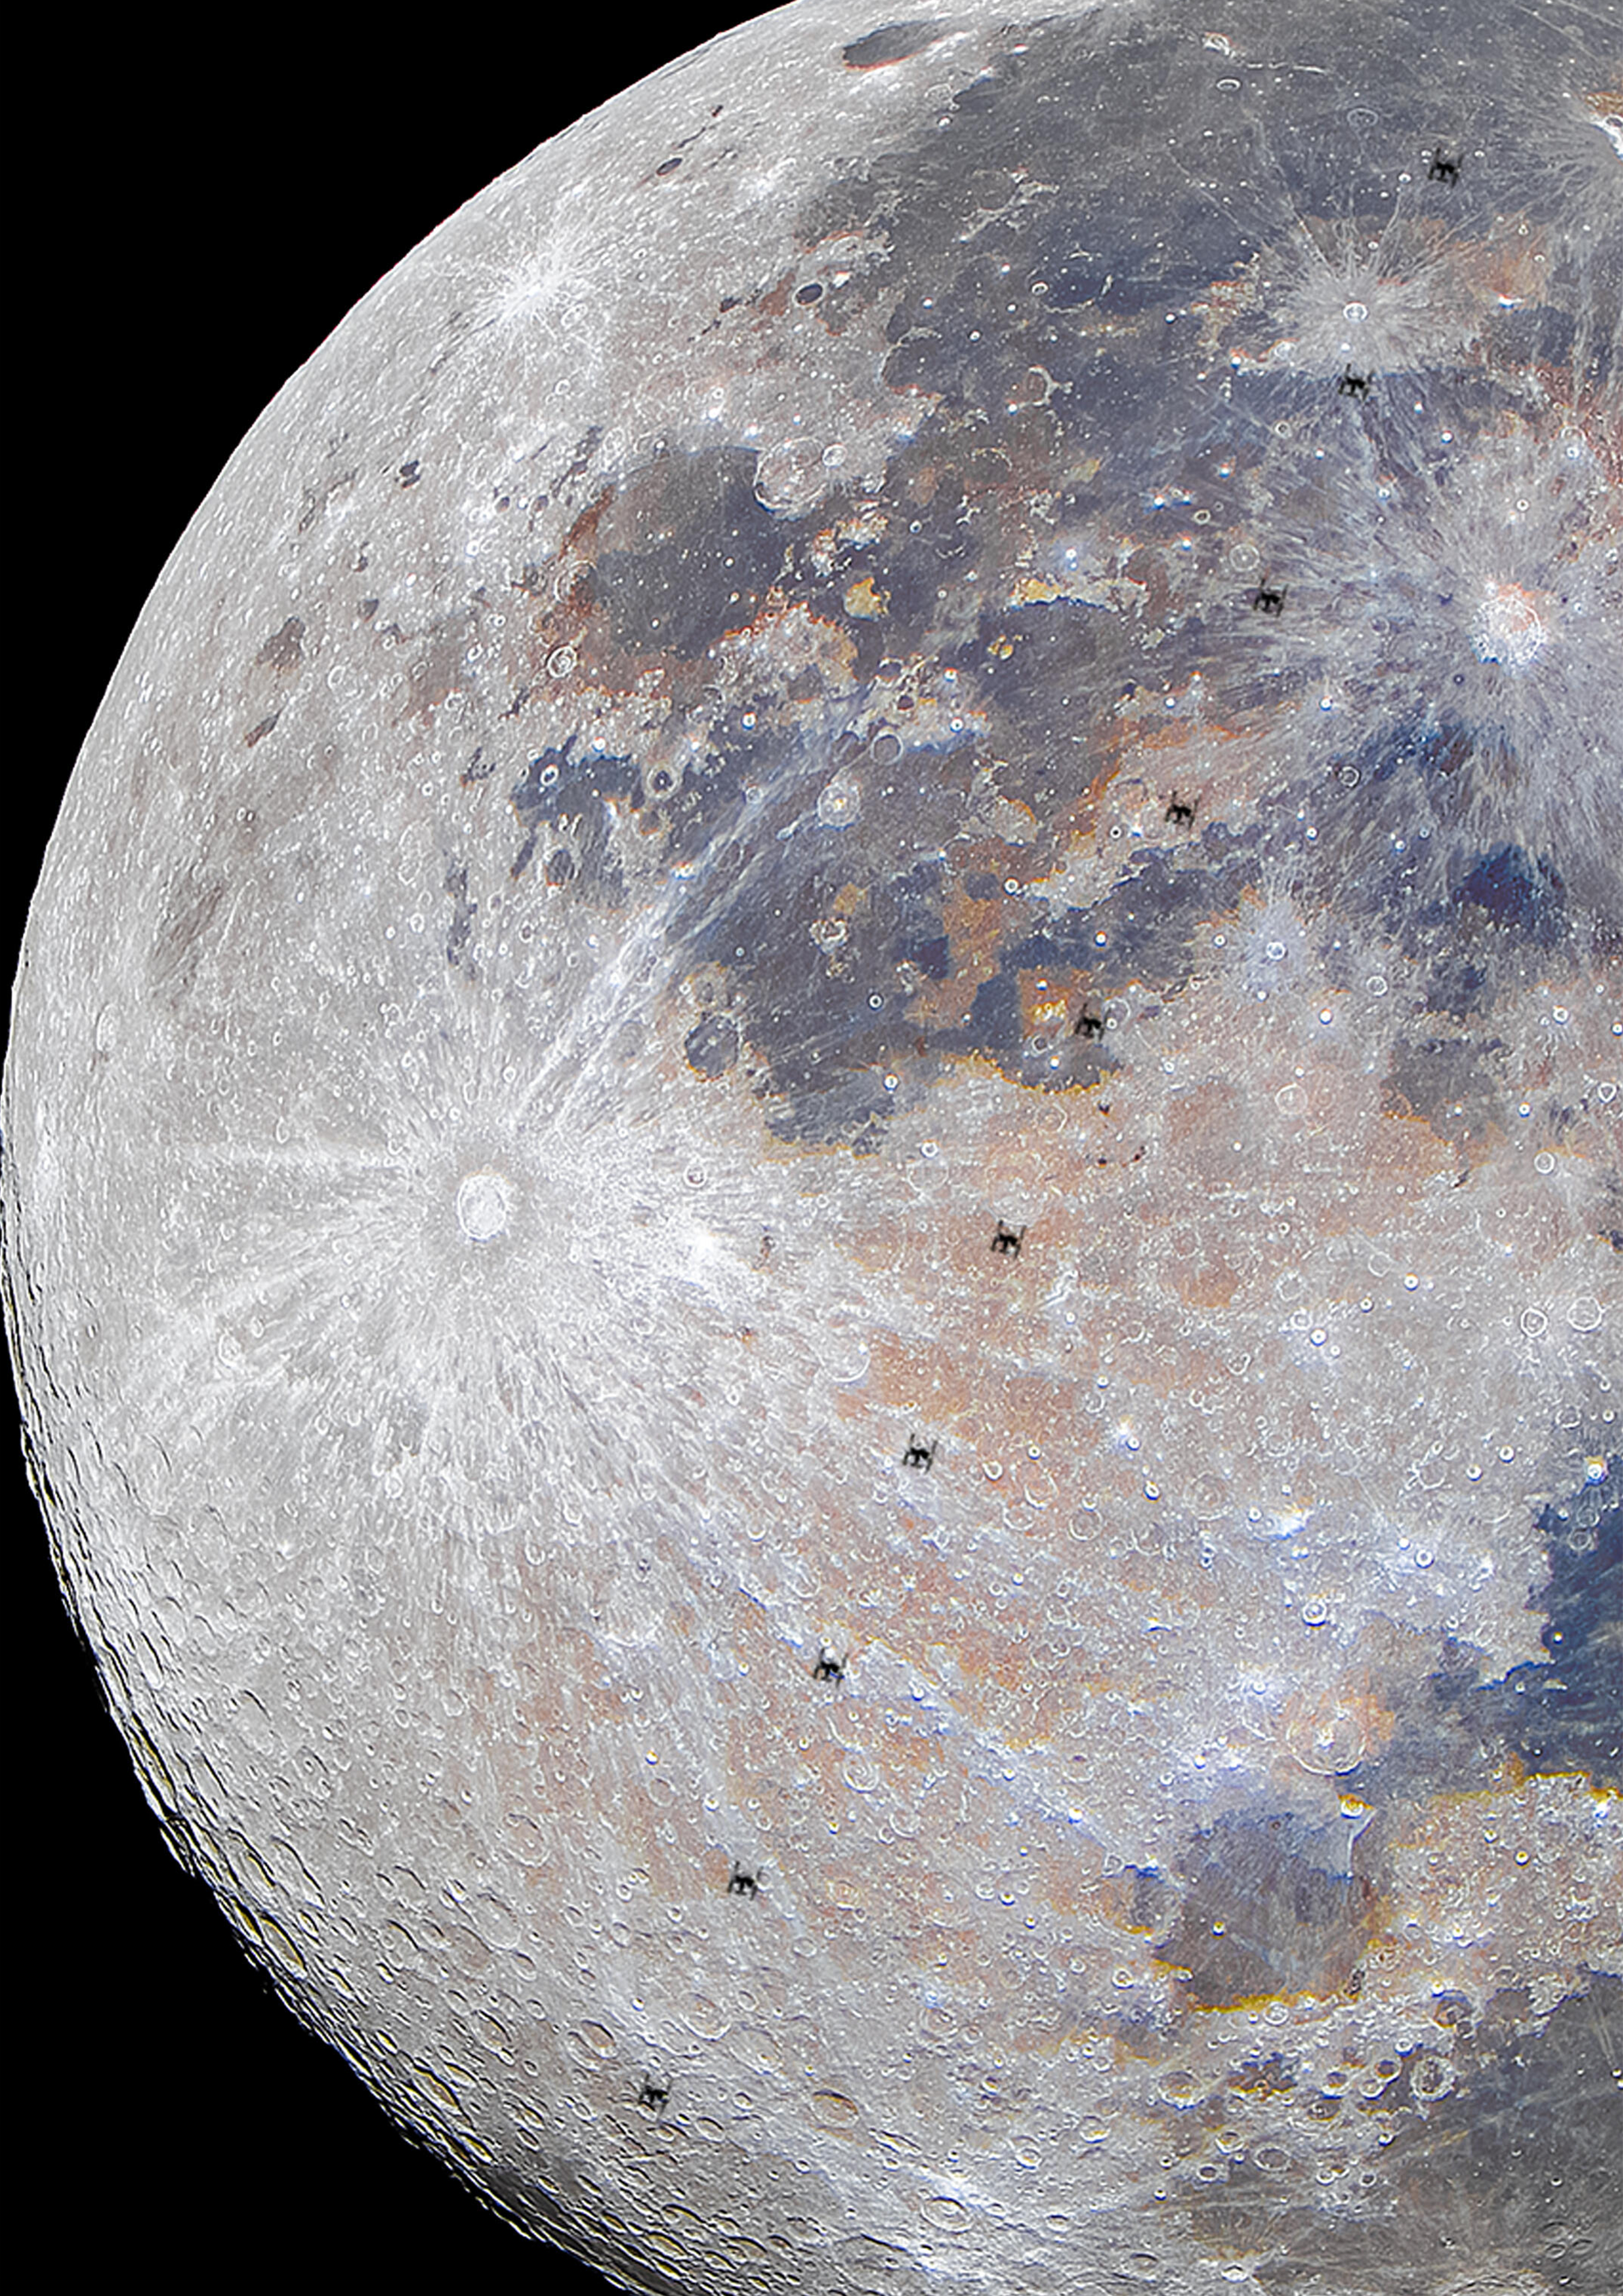
\includegraphics[width=\paperwidth,height=\paperheight]{img/background_letter.png}}, % 图片路径(你后续替换),铺满整页
  scale=1,            % 图片缩放比例固定1,不拉伸
  angle=0,            % 图片旋转角度0,不旋转
  opacity=0.22           % 图片透明度1(完全不透明,需调淡可改0.8/0.9)
}
\BgThispage % 核心命令:仅将上述背景应用于「当前备忘录页面」

% 以下为信件/备忘录部分,不需要可自行去掉========================================================================
% 如有需要可将整个 letter 环境移动到文章开头或中间
% 请在第二个花括号内填写标题,如「信件」(Letter)或「备忘录」(Memorandum)
\begin{letter}{Letter}
	\begin{flushleft}  % 左对齐环境,无首行缩进
		\textbf{To:} Moon Base Management (MCM) Agency\\
		\textbf{From:} Team 2615409\\
		\textbf{Date:} February 1st, 2026\\
		\textbf{Subject:} Proposal for the 2050 Lunar Base Construction and Operation Mission
	\end{flushleft}

Greetings. Based on multi-dimensional modeling and feasibility analysis, we hereby recommend a comprehensive strategy for the 100,000-person lunar base, balancing efficiency, cost-effectiveness, robustness, and environmental sustainability.

\begin{enumerate}
	\item Optimization: Our \textbf{Hybrid Dynamic Transportation Mode}, integrated with a \textbf{Time-Adaptive Dynamic Expansion Model} to optimize $\alpha(i)$ allocation, outperforms static and single-mode approaches. This strategy compresses the timeline to approximately 380 years while significantly reducing costs.This approach demonstrates superior performance over single or static transportation modes when evaluated under the dual-objective constraints of time and cost.
	\item Robustness: We incorporate \textbf{rigorous risk correction}. Transfer Rocket (TR) capacity is derated for launch failure probabilities. Space Elevator (SE) stability is secured via a Weibull distribution wind model to establish oscillation thresholds. By integrating maintenance downtime coefficients and apical rocket launch success rates, the corrected model ensures a \textbf{stable and reliable} supply chain.
	\item Resources: Addressing the projected 638.75k-ton annual water demand, we recommend a \textbf{"Transportation + Recycling"} model to maximize cost-efficiency.
	\item Futhermore: Pareto Frontier Analysis is employed to optimize trade-offs between operational goals and \textbf{Earth's ecological preservation}, achieving a global optimum for the comprehensive objective function.
\end{enumerate}

This proposal offers superior feasibility, verified robustness, and low-carbon sustainability. We remain at your disposal for further model refinement and are dedicated to advancing human space exploration.


\end{letter}

%=================================================================================================================
\newpage
%===============================================参考文献部分=============================================
\backgroundsetup{contents={}} 


%=====================================================================================



% 以下为附录内容
% 如您的论文中不需要附录,请自行删除
\begin{subappendices}  % 附录环境开始
	\section{Appendix C: Report on Use of AI}
	% 人工智能的报告
	1. OpenAI ChatGPT (Nov 5, 2023 version, ChatGPT-4)

	Query1: <insert the exact wording you input into the AI tool>
	
	Output: <insert the complete output from the AI tool>

	2. OpenAI Ernie (Nov 5, 2023 version, Ernie 4.0)
	
	Query1: <insert the exact wording of any subsequent input into the AI tool>
	
	Output: <insert the complete output from the second query>
	
	3. Github CoPilot (Feb 3, 2024 version)
	
	Query1: <insert the exact wording you input into the AI tool>
	
	Output: <insert the complete output from the AI tool>
	
	4. Google Bard (Feb 2, 2024 version)
	
	Query: <insert the exact wording of your query>
	
	Output: <insert the complete output from the AI tool>
	

\end{subappendices}  % 附录内容结束

\end{document}  % 结束
